\documentclass{article}
\usepackage[utf8]{inputenc}
\usepackage[margin=1in]{geometry}
\usepackage{graphicx}
\usepackage{natbib}
\usepackage{enumitem}
\usepackage{array}
\usepackage{gensymb}
\usepackage{indentfirst}
\graphicspath{ {Images/} }
\usepackage{float}
\usepackage[table,xcdraw]{xcolor}

\title{Physics 111A Fall 2016- Lab 6\\
Op Amps I}
\author{Joshua Levy\\Lab Partner: Alex Chuang}
\date{October 9th, 2016}


\begin{document}

\maketitle

\section{Lab Write Up}

%1
\subsection{Comparators}
    \begin{figure}[H]
        \centering
        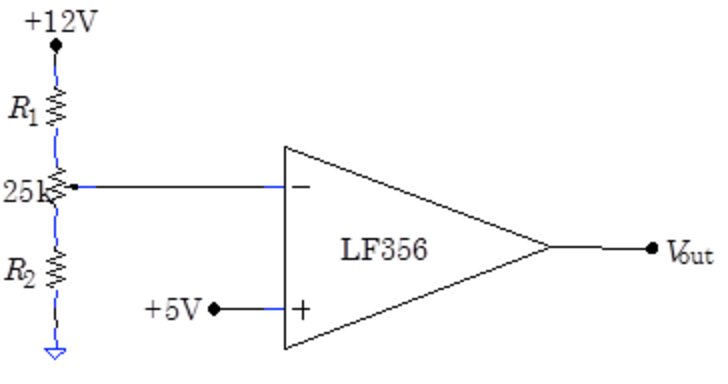
\includegraphics[scale = 0.5]{1.png}
        \caption{Comparator ~\cite{webfig}}
        \label{fig:my_label}
    \end{figure}
    \begin{figure}[H]
        \centering
        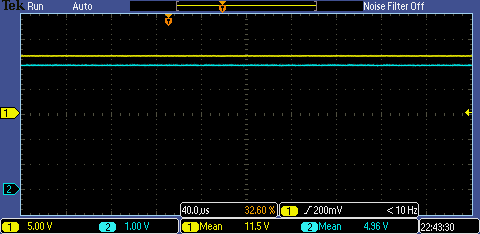
\includegraphics[scale = 0.7]{1a.PNG}
        \caption{$V_{out}$ of comparator for $V_- < V_+$}
        \label{fig:my_label}
    \end{figure}
    \begin{figure}[H]
        \centering
        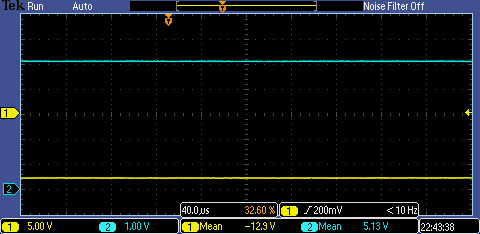
\includegraphics[scale = 0.7]{1b.PNG}
        \caption{$V_{out}$ of comparator for $V_- > V_+$}
        \label{fig:my_label}
    \end{figure}
    \begin{figure}[H]
        \centering
        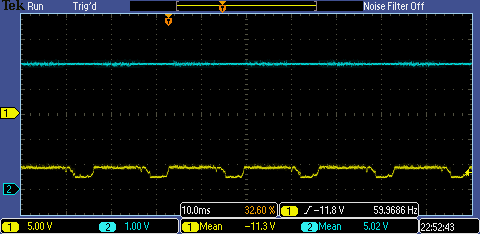
\includegraphics[scale = 0.7]{1c.PNG}
        \caption{Fluctuations of Comparator as $V_- \rightarrow 5V$}
        \label{fig:my_label}
    \end{figure}
    We built the circuit featured in figure 1, set $V_+$ to +5V, and adjusted the potentiometer voltage through +5V. Producing the output image traces as depicted on figures 2 and 3. Channel 1 is the comparator output and channel 2 is the potentiometer voltage $V_-$. We see that when $V_-$ is less than $V_+$ (figure 2), $V_{out}$ is pretty much 12 V. When $V_-$ is more than $V_+$ (figure 3), the output drops to -12V. We were not able to adjust the potentiometer to voltages intermediate to $\pm$12V. As we adjusted the potentiometer just to that it was hovering near 5V, the output would either be +12V or -12V. It is really hard to get an intermediate value in this scenario because although there is a small $V_-$ region where $V_{out}$ can take on intermediate values, this region is very small, pretty much at 0, (partially because of the lack of external resistors), and thus, as you try to change $V_-$ to $V_+$, you'll always be off by some noticeable amount, and the result will yield a $V_{out}$ of $\pm12V$. 
    \\\indent Now, if we imagine that the gain of our system is our differential gain:
    \begin{equation}
        G = \frac{V_{out}}{V_+ - V_-}
    \end{equation}
    We can set $V_+$ to be +5V, and let us denote $V_-$ as $x$, with $x \in [0,12](volts)$. If x $<$ 5, $V_{out}$ is 12V, if 5 $<$ x $<$ 12, $V_{out}$ is -12V. Thus, we can rewrite the equation for the gain as:
    \begin{equation}
        \begin{array}{llll}
            G & = & \frac{12}{5-x} & x \in [0,5] \\
            G & = & \frac{-12}{5-x} & x \in [5,12]
        \end{array}
    \end{equation}
    Evaluating the endpoints (x=0 and x=12) and we see that the gain here is $\frac{12}{5}$ and $\frac{12}{7}$ respectively. Evaluating x=5, and we see the gain G$\rightarrow \infty$. Thus, the lower bound limit on the gain is $\frac{12}{7}$ when you set $V_-$ to +12V. However, if we try to bring $V_+$ as close together to $V_-$, the denominator of eq.(2) becomes .001V, and we can estimate our lowest bound on the differential gain to be $\approx$ 12kV.
    \\\indent Moving onwards, we set the $R_1$ and $R_2$ values such that $R_1 > R_2$, and tweaked the potentiometer so that $V_-$ hovered around +5V (figure 4). We noticed fluctuations in the output signal (figure 4, channel 1) that triggered in at 59.9686 Hz after we had performed line-syncing. This shows that the fluctuations were approximately at 60Hz, that of the power supply source.
    
%2
\subsection{Hysteric Comparator}
    See Signature Page.
%3
\subsection{Follower}
    \begin{figure}[H]
        \centering
        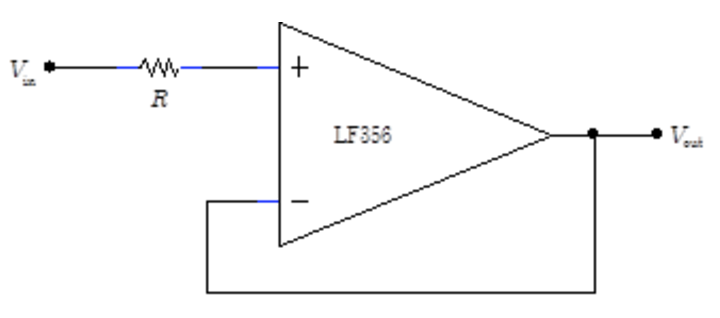
\includegraphics[scale = 0.5]{3.png}
        \caption{Follower ~\cite{webfig}}
        \label{fig:my_label}
    \end{figure}
    We constructed the follower depicted in figure 5. After investigating the follower's performance for a variety of input signals of different shapes, frequencies, and amplitudes, the follower appeared to perform as a JFET source follower without R being inserted into the circuit. With a 1 $V_{pp}$, 1 kHz sine wave input we recorded the following gains for various resistor (R) values:
    \begin{table}[H]
        \centering
        \caption{Follower Gains with Various R-Values}
        \label{my-label}
        \begin{tabular}{ccccc}
        \textbf{$R_{meas}(\Omega)$} & \textbf{$R_{ideal}(\Omega)$} & \textbf{$V_{in}$(V)} & \textbf{$V_{out}$(V)} & \textbf{Gain} \\ \hline
        101 & 100 & 1.005 & 1.021 & 1.015920398 \\
        971 & 1000 & 1 & 1 & 1 \\
        9990 & 10000 & 1 & 1 & 1 \\
        9960 & 100000 & 1 & 1 & 1 \\
        9993000 & 10000000 & 1 & 0.923 & 0.923 \\
        986000 & 1000000 & 1.005 & 1.028 & 1.022885572
        \end{tabular}
    \end{table}
    As noticed in the above table, the gain begins to drop off at R $\approx$ 10M and we indeed begin seeing anomalies in out follower (the gain begins to decrease). Treating the follower as a black box, we can imagine a circuit as a voltage divider in which R is in the upper leg and $Z_{in}$, the input impedance of the follower, is in the lower leg. Thus, the gain of the circuit is:
    \begin{equation}
        G = \frac{V_{out}}{V_{in}} \approx \frac{Z_{in}}{Z_{in} + R}
    \end{equation}
    $Z_{in}$ is normally large compared to R, but at R-values approaching 10M, we see that the two are on similar orders of magnitude. Setting R equal to 9.93 M, and G = 0.923 (where the gain begins to decrease) from the data in the above figure, we can find a relatively low bound on the input impedance, as we rework eq.(1) to find:
    \begin{equation}
        Z_{in}lower \approx \frac{R*G}{1-G} = \frac{9.93M * 0.923}{1-0.923} \approx 119.03 M\Omega
    \end{equation}
    Changing the frequency of our input signal to 50 Hz, and we find that with the 10M resistor, that $V_{in} = V_{out} = 1.0V$, so the anomalies go away at a lower frequency.
%4
\subsection{Inverting Amplifier}
    See signature page.
%5
\subsection{Non-Inverting Amplifier}
    \begin{figure}[H]
        \centering
        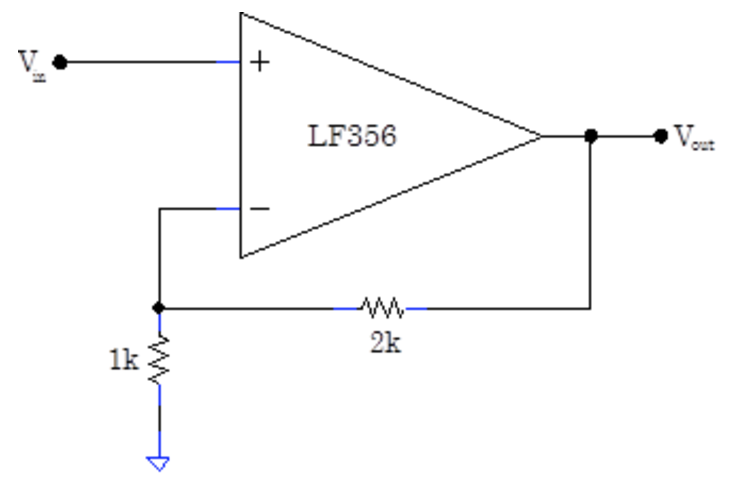
\includegraphics[scale = 0.5]{5.png}
        \caption{Non-Inverting Amplifier ~\cite{webfig}}
        \label{fig:my_label}
    \end{figure}
    We built the non-inverting amplifier above and the 1k resistor measured to be 0.971k and the 2k resistor measured to be 1.97k. In our prelab, we expected the circuit gain to be 3 ($G_{design}$ = 3), however, in this case, with the measured resistor values, the predicted gain is:
    \begin{equation}
        G_p = \frac{R_{2k}}{R_{1k}} + 1 = \frac{1.97k}{0.971k} + 1 = 3.029
    \end{equation}
    which was found by utilizing the two op amp golden rules, which led us to the relationship:
    \begin{equation}
        \frac{V_{out} - V_{in}}{R_2} = \frac{V_{in}}{R_1}
    \end{equation}
    which rearranged produces the first part of $G_p$. With these values in mind, we measured $V_{in} = 200 mV$ and $V_{out}$ = 628.3 mV, yielding an actual gain of $G_{exp} = \frac{628.3}{200} \approx 3.1415$.\\\indent In comparing the design gain $G_{design}$ with the experimental gain $G_{exp}$, we yield a relative error of:
    \begin{equation}
        RelError = |\frac{G_{exp} - G_{design}}{G_{design}}| * 100\% = \frac{3.1415 - 3}{3} * 100\% \approx 4.72\%
    \end{equation}
    For the comparison between the predicted gain with the measured resistor values and the experimental gain, we see that the relative error is:
    \begin{equation}
        RelError = |\frac{G_{exp} - G_{p}}{G_{p}}| * 100\% = \frac{3.1415 - 3.029}{3.029} * 100\% \approx 3.71\%
    \end{equation}
    The experimental gain $G_{exp}$ is quite close to the predicted and design gain values.
%6
\subsection{The Virtues of Feedback}
    \begin{figure}[H]
        \centering
        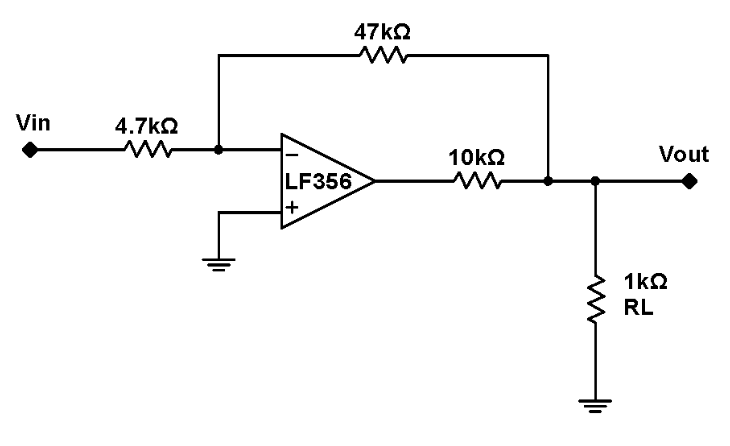
\includegraphics[scale = 0.5]{6.png}
        \caption{Feedback Circuit 0 ~\cite{webfig}}
        \label{fig:my_label}
    \end{figure}
    Building the inverting amplifier seen above, we measured the 10k resistor to be 9.99k, the 1k load resistor ($R_L$) to be 0.971k, the 4.7k resistor to be 4.69k, and the 47k resistor to be 46.9k.\\\indent With $R_L$ removed, and for a 0.1 $V_{pp}$, 1kHz input sine wave, $V_{in} = 100.7 mV$, $V_{out} = 1.005 V$, and we find a gain of $\frac{1005}{100.7} \approx 9.98$; changing to a 1$V_{pp}$ input signal, $V_{in} = 1.006 V$, $V_{out} = 10 V$, and we find a gain of $\frac{10.}{1.006} \approx 9.94$. Due to Op Amp Golden Rule 2 ~\cite{webfig}, the input does not draw any current, and so the current flows around the op amp and through the 47k resistor but skips over the 10k resistor. Without $R_L$ inserted, and we see that the current flows directly through $V_{out}$. Thus, utilizing the circuit gain relation found in the lab's background ~\cite{webfig}, the absolute value of our predicted gain is $G_p = \frac{R_{47k}}{R_{4.7k}} = \frac{46.9k}{4.68k} \approx 10.02$. Thus, with measured gains around 10, the gain is what we expect for both cases.
    \\\indent With $R_L$ inserted into the circuit, and for a 0.1 $V_{pp}$, 1kHz input sine wave, $V_{in} = 0.1 V$, $V_{out} = 1 V$, and we find a gain of $10$; changing to a 1$V_{pp}$ input signal, $V_{in} = 0.98 V$, $V_{out} = 2 V$, and we find a gain of $\frac{2.}{0.98} \approx 2.04$. However, the output of the 1$V_{pp}$ input signal, with $R_L$ included in the circuit, is no longer a sine wave but looks more like a square wave, as shown in the figure below:
    \begin{figure}[H]
        \centering
        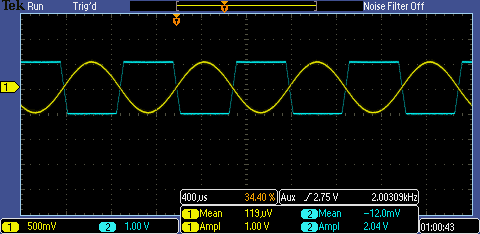
\includegraphics[scale = 0.7]{6a.PNG}
        \caption{"Broken" Circuit with a load resistor and 1 $V_{pp}$ input sine signal}
        \label{fig:my_label}
    \end{figure}
    In this case, we see that the amplifier does not work for both input voltages. It works for a 0.1$V_{pp}$ input signal but not for the 1$V_{pp}$ input signal. The gain is roughly the same for the 0.1$V_{pp}$ input signal, regardless if $R_L$ was included, but was different for the 1$V_{pp}$ input signal, and we should dismiss the 1$V_{pp}$ input signal with $R_L$ included because the output signal is distorted. The reason for the circuit failure at 1$V_{pp}$ with the load resistor is because the feedback pushes the output voltage of the Op Amp into saturation. Judging from our predicted gain of $\sim$ -10, we would expect the output of a 1 $V_{pp}$ wave to be 10V. The presence of the load resistor pushes the direct output of the Op Amp ($V_o$) (before some voltage is dropped across the 10k resistor) to be higher than the power supply voltage, and thus figure 8 depicts the output getting cutoff at values outside $\pm$1V after the voltage is dropped across the 10k resistor. We can use a voltage divider relation on between the direct output of the op amp (denote as $V_o$) and the right ground of figure 7 to yield the actual $V_{out}$ of $V_o*\frac{1k}{10k + 1k}$. Setting $V_{out} = 2V$, the conditions that we found under the failure, and we can estimate $V_o$ to be 22V. This far exceeds the power supply of the op amp and we see that we have a circuit failure for 1$V_{pp}$ input with the load resistor. 
%7
\subsection{Even More Virtues of Feedback - I}
    \begin{figure}[H]
        \centering
        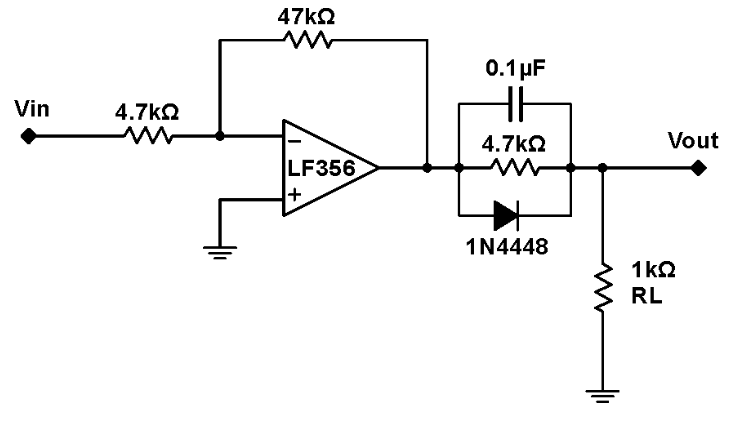
\includegraphics[scale = 0.5]{7.png}
        \caption{Feedback Circuit I ~\cite{webfig}}
        \label{fig:my_label}
    \end{figure}
    \begin{figure}[H]
        \centering
        a)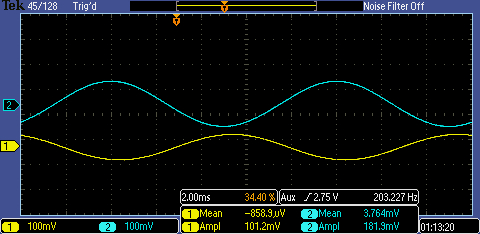
\includegraphics[scale = 0.7]{7d.PNG}
        b)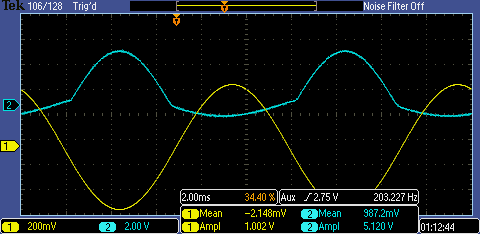
\includegraphics[scale = 0.7]{7c.PNG}
        \caption{Feedback Circuit I (figure 9)(output is channel 2), driven @ 100 Hz with: a) 0.1 $V_{pp}$ sine wave; b) 1 $V_{pp}$ sine wave}
        \label{fig:my_label}
    \end{figure}
    \begin{figure}[H]
        \centering
        a)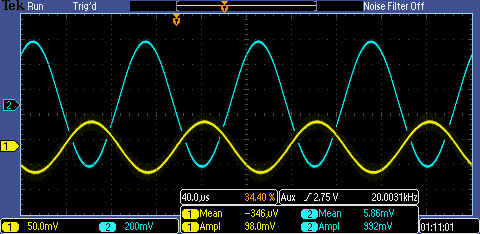
\includegraphics[scale = 0.7]{7a.PNG}
        b)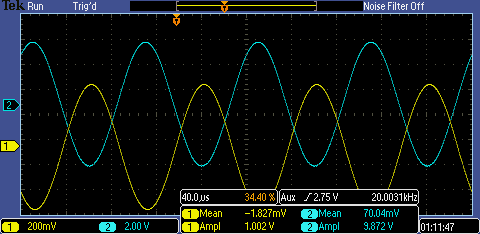
\includegraphics[scale = 0.7]{7b.PNG}
        \caption{Feedback Circuit I (figure 9)(output is channel 2), driven @ 10 kHz with: a) 0.1 $V_{pp}$ sine wave; b) 1 $V_{pp}$ sine wave}
        \label{fig:my_label}
    \end{figure}
    The feedback circuit constructed from figure 12 uses the resistor values used in the previous sections, but also includes a diode, a 4.7k resistor $R_{4.7k2}$ that measured in at 4.63k and a 0.1 $\mu$F that measured to be 105.7 nF. Above (figures 10 and 11) are images of the circuit output at 100 Hz and 10 kHz. Figure 10b demonstrates a distorted output signal when the circuit is driven with a 1 $V_{pp}$ input signal at 100 Hz. This is to suggest that the circuit becomes non-linear at a combination of low frequencies and larger voltages. First, we notice that our output image is inverted from the input via the op amp inverted amplification. However, any values below around 0V for this inverted signal appear to be almost rectified by the diode. Nevertheless, this "rectification" only occurs at low frequencies, so the capacitor seems to bypass the inverted high frequency high voltage amplitude signals. Figure 11b demonstrates this effect, as the 1$V_{pp}$ input waves that had their inverted and amplified waves rectified at low frequencies seem to be untouched at high frequencies. To reiterate, the diode-capacitor interaction effect will only rectify waves that are at low frequency high voltage amplitude.
    
%8
\subsection{Even More Virtues of Feedback - II}
    \begin{figure}[H]
        \centering
        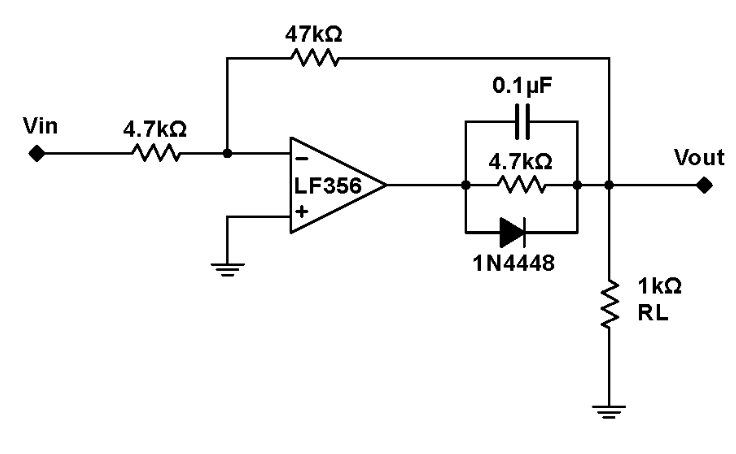
\includegraphics[scale = 0.5]{8.png}
        \caption{Feedback Circuit II ~\cite{webfig}}
        \label{fig:my_label}
    \end{figure}
    \begin{figure}[H]
        \centering
        a)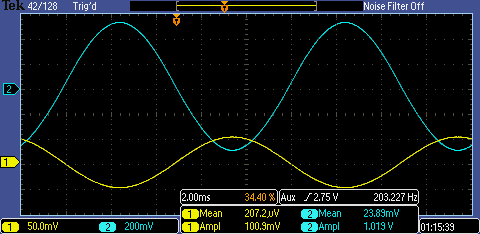
\includegraphics[scale = 0.7]{8a.PNG}
        b)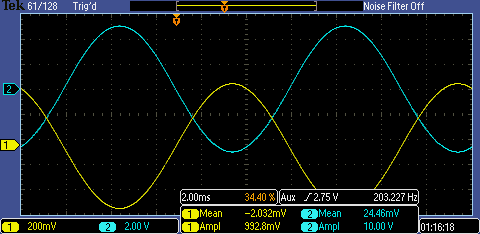
\includegraphics[scale = 0.7]{8b.PNG}
        \caption{Feedback Circuit II (figure 12)(output is channel 2), driven @ 100 Hz with: a) 0.1 $V_{pp}$ sine wave; b) 1 $V_{pp}$ sine wave}
        \label{fig:my_label}
    \end{figure}
    \begin{figure}[H]
        \centering
        a)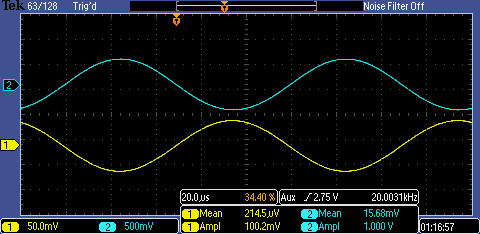
\includegraphics[scale = 0.7]{8c.PNG}
        b)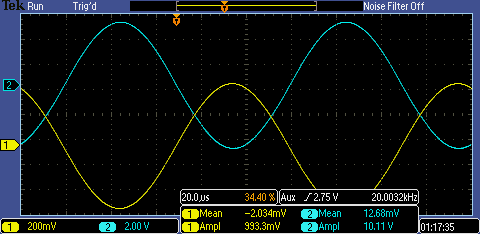
\includegraphics[scale = 0.7]{8d.PNG}
        \caption{Feedback Circuit II (figure 12)(output is channel 2), driven @ 10 kHz with: a) 0.1 $V_{pp}$ sine wave; b) 1 $V_{pp}$ sine wave}
        \label{fig:my_label}
    \end{figure}
    With the same resistors, op amp, capacitor, and diode used as in the previous section, but with the circuit setup of figure 12, we attain the following $V_{in}$, $V_{out}$, and gain:
    \begin{table}[H]
        \centering
        \caption{Gain of Feedback Circuit II Across Various Conditions}
        \label{my-label}
        \begin{tabular}{llll}
        \textbf{f (Hz)} & \textbf{$V_{in}$(V)} & \textbf{$V_{out}$(V)} & \textbf{Gain} \\ \hline
        100 & 0.1009 & 1.019 & 10.09910803 \\
        10000 & 0.1002 & 1 & 9.98003992 \\
        100 & 0.9928 & 10 & 10.07252216 \\
        10000 & 0.9933 & 10.11 & 10.1781939
        \end{tabular}
    \end{table}
    These values were found from observing the outputs of figures 13 and 14. In this case, we see that the circuit is now no longer frequency dependent, and is now a linear circuit, producing output signals with a gain of approximately 10 and retaining the same sine wave shape as its input signal. However, the output signals have been inverted. Now, the circuit is no longer broken at 1 $V_{pp}$ with the load resistor as in part [1.6] and is no longer frequency dependant and nonlinear as in part [1.7].
    
%9
\subsection{Differential Amplifier}
    See signature page.
%10
\subsection{Summing Amplifier}
    \begin{figure}[H]
        \centering
        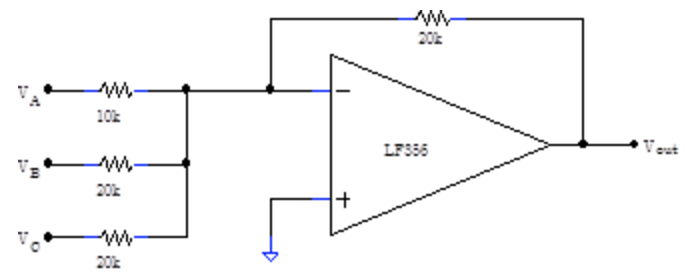
\includegraphics[scale = 0.7]{10.png}
        \caption{Summing Amplifier ~\cite{webfig}}
        \label{fig:my_label}
    \end{figure}
    We constructed the summing amplifier above, measuring the 10k resistor near $V_A$ to be 9.9k, the 20k resistor near $V_B$ to be 20.7k, the 20k resistor near $V_C$ to be 20.6k, and the other 20k resistor to be 19.4k. A resistor of arbitrary value was attached between the $V_A$ and $V_B$ points, and another resistor of arbitrary value was attached between $V_B$ and $V_C$ (see figure 15). A 1$V_{pp}$ sine wave input was fed into $V_A$ and the voltages $V_B$ and $V_C$ were generated through voltage drops across each of the two arbitrary resistors. We can now treat the system as if we have three separate power sources, where $V_A$ was measured to be 960 mV, $V_B$ was measured to be 832 mV, and $V_A$ was measured to be 784 mV (all measurements are peak-peak). The output signal was measured to be 3.76V $V_{pp}$. We will denote $V_{out}$ = -3.76V $V_{pp}$, as the minus sign is for the inversion of the signal with respect to the input.\\\indent Out predicted $V_{out}$ is ~\cite{webfig}:
    \begin{equation}
        V_{out}^{predicted} = -(2V_A + V_B + V_C) = -(2*0.96 + 0.832 +0.784)V \approx -3.536
    \end{equation}
    We see that the relative error between the predicted $V_{out}$ and the measured $V_{out}$ is:
    \begin{equation}
        Error_{Relative} = |\frac{V_{out}^{predicted} - V_{out}^{measured}}{V_{out}^{predicted}}| * 100\% = \frac{3.76-3.536}{3.536} * 100\% \approx 6.33\%
    \end{equation}
    So we see that the measured output of the circuit is roughly equal to the value predicted by eq.(9).
%11
\subsection{Current to Voltage Converters}
    See Signature Page.
%12
\subsection{Op Amp Current Source}
    \begin{figure}[H]
        \centering
        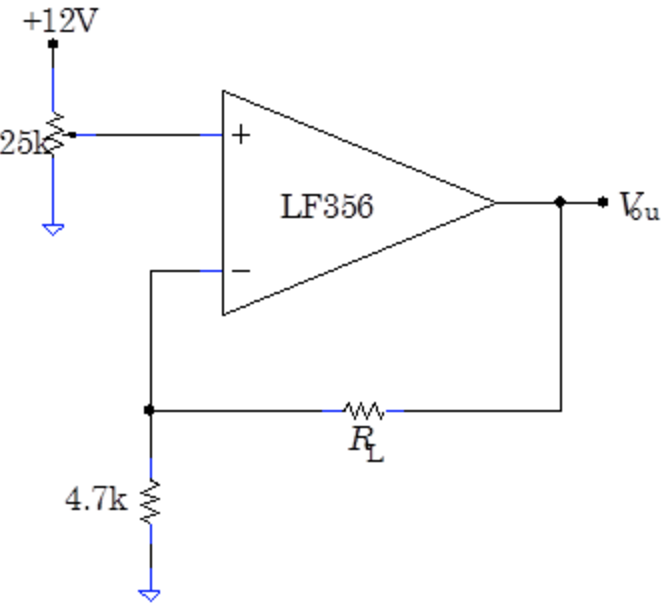
\includegraphics[scale = 0.5]{12.png}
        \caption{Op Amp Current Source ~\cite{webfig}}
        \label{fig:my_label}
    \end{figure}
    My partner and I built the op amp current source pictured above and measured the 4.7k resistor to be 4.68k. After setting the potentiometer output to +3V, we measured the current through load resistor $R_L$. For $R_L = 4.7k$, which was actually measured to be 4.63k, we measured the current to be 0.7 mA. For various load resistor resistances, we find the following currents:
    \begin{table}[H]
        \centering
        \caption{Op Amp Current Source Output Currents for Various $R_L$ values}
        \label{my-label}
        \begin{tabular}{cc}
        \textbf{$R_L (\Omega)$} & \textbf{Current I (mA)} \\ \hline
        100 & 0.706 \\
        100 & 0.706 \\
        1020 & 0.7 \\
        2020 & 0.7 \\
        4600 & 0.7 \\
        4630 & 0.7 \\
        9880 & 0.706 \\
        19900 & 0.627 \\
        51600 & 0.26 \\
        100000 & 0.107
        \end{tabular}
    \end{table}
    We notice the current begins to noticeably dip at $R_L$ = 19.9k, where the current is 0.627 mA instead of the nominal 0.7 mA. So we see that the range of $R_L$ over which the current does not vary significantly is between 100$\Omega$ and around 19k although we can interpolate the actual point by which the current drop is significant to be somewhere in between 10k and 19k.\\\indent We restored the load resistor to be about 4.7k (measured to be 4.67k), and varied the potentiometer voltage and found the following current values:
    \begin{table}[H]
        \centering
        \caption{Op Amp Current Source Output Currents for Various $V_{potentiometer}$ values}
        \label{my-label}
        \begin{tabular}{cc}
        \multicolumn{1}{l}{\textbf{$R_L$ = 4.67k}} & \multicolumn{1}{l}{\textbf{}} \\
        \textbf{$V_{potentiometer}$ (V)} & \textbf{I (mA)} \\ \hline
        0 & 0.0005 \\
        2 & 0.44 \\
        4 & 0.855 \\
        6 & 1.23 \\
        8 & 1.23 \\
        10 & 1.23 \\
        12 & 1.23
        \end{tabular}
    \end{table}
    Of course, the data displays the magnitude of current measured. The data is plotted on the following chart:
    \begin{figure}[H]
        \centering
        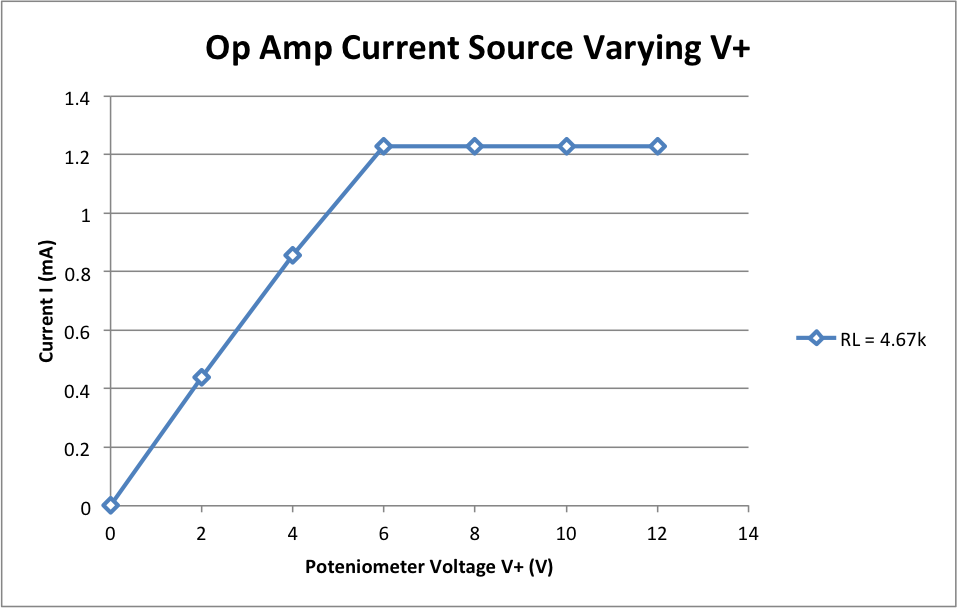
\includegraphics[scale = 0.5]{12a.png}
        \caption{Op Amp Current Source Output Currents plot for Various $V_{potentiometer}$ values}
        \label{fig:my_label}
    \end{figure}
    And fitting a trendline to the points that exist between $V_{potentiometer}$ = 0 V and $V_{potentiometer}$ = 6 V and we find a nicely fitting linear trend:
    \begin{equation}
        I = 0.2052V_+ + 0.0159
    \end{equation}
    with a correlational $R^{2}$ value of 0.99875. For points past $V_{potentiometer}$ = 6 V, the current line flattens out. So we can see that as the voltage coming into $V_+$ increases, the magnitude of the current increases by a proportional amount, clearly indicative that this circuit can also serve as a current to voltage converter across a certain domain. The current that has been set by the potentiometer voltage serves as a constant current source that will maintain a constant current across many different changes to the circuit.
    
    
%13
\subsection{Output Impedance Calculation}
    \begin{figure}[H]
        \centering
        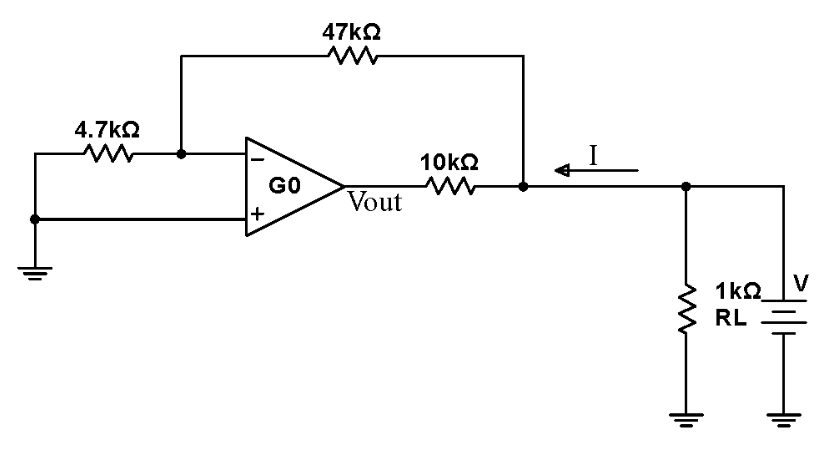
\includegraphics[scale = 0.5]{13.png}
        \caption{Reimagined Circuit from [1.6] ~\cite{webfig}}
        \label{fig:my_label}
    \end{figure}
    \begin{figure}[H]
        \centering
        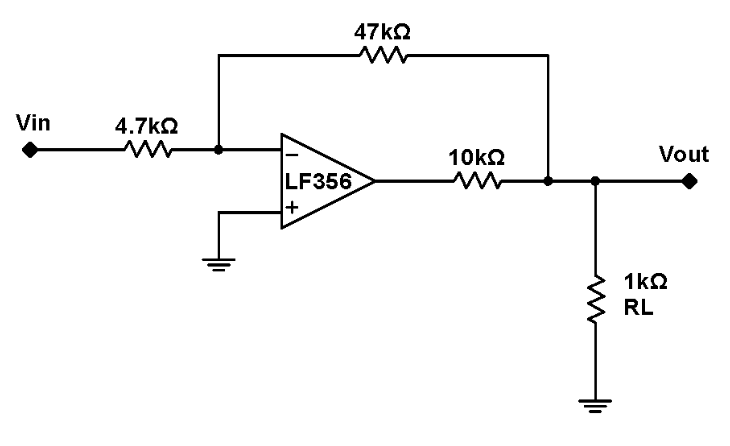
\includegraphics[scale = 0.5]{6.png}
        \caption{Repictured [1.6] Circuit ~\cite{webfig}}
        \label{fig:my_label}
    \end{figure}
    We are seeking to find the output impedance $Z_{out}$ of the amplifier of section [1.6], and the equivalent circuit of figure 7 (repictured as figure 19) is figure 18, pictured above. And we know~\cite{webfig}:
    \begin{equation}
        Z_{out} = \frac{V}{I}
    \end{equation}
    We know by the Op Amp Golden Rules ~\cite{webfig} that $V_- \approx V_+ = 0V$. Also given is ~\cite{webfig}:
    \begin{equation}
        V_{out} = -G*V_-
    \end{equation}
    where G is open-loop gain, so $V_-$ is not actually 0V. It is found through the voltage divider relation: 
    \begin{equation}
        V_- = \frac{4.7k}{4.7k + 47k} * V = \frac{V}{11}
    \end{equation}
    So $V_{out} = -G*\frac{V}{11}$. We also know that the leftward current I, can be broken up into the current passing through the 10k resistor, $i_{10k}$ and the current passing through the feedback resistor $i_f$. So:
    \begin{equation}
        I = i_f + i_{10k}
    \end{equation}
    Using the $V_{out}$ from figure 18, and we see that the voltage drop across the 10k resistor is:
    \begin{equation}
        V - V_{out} = i_{10k} * 10k
    \end{equation}
    and after rearranging and substituting for $V_{out}$:
    \begin{equation}
        i_{10k} = \frac{V * (1 + \frac{G}{11})}{10k} 
    \end{equation}
    Now, under the assumption that $V_- \approx V_+ = 0V$, we can calculate $i_f$ to be:
    \begin{equation}
        i_f = \frac{V}{47k}
    \end{equation}
    Substituting eqs.(17,18) into eq.(15), and we find that:
    \begin{equation}
        I \approx V * (\frac{1 + \frac{G}{11}}{10k} + \frac{1}{47k})
    \end{equation}
    And thus, substituting this back into eq.(12) and rearranging:
    \begin{equation}
        Z_{out} = (\frac{1}{10k} + \frac{1}{47k} + \frac{G}{110k})^{-1} = \frac{1}{\frac{1}{10k} + \frac{1}{47k} + \frac{G}{110k}}
    \end{equation}
    We note that typically, G has very large values in the millions, so we take the high G limit, which eliminates the other two values without G in the denominator of the above equation:
    \begin{equation}
        Z_{out} \approx \frac{110k}{G}
    \end{equation}
    Because the open loop gain G has such a high value, we expect this output impedance to be quite small. 
    \\\indent The Op Amp fails under certain conditions when the circuit is loaded because the low output impedance has only a negligible effect on the voltage divider relation established by the 10k resistor and the 1k load resistor. Through such a relation, we see that the presence of the load causes a large increase in the direct output of the op amp before any voltage is dropped across the 10k resistor. In section [1.6] we showed how under certain $V_{in}$ conditions, the circuit fails with a given load resistor, and this is true, because $V_o$ (see part [1.6], this is the direct output of the op amp) is equal to $V_{out} \frac{10k + R_L}{R_L}$, so $V_o$ is larger than $V_{out}$ and can exceed the power supply for a given gain. This will cause the circuit to fail as the direct output of the op amp reaches the saturation region.
%14
\subsection{Summing Amplifier Calculation}
    Referring back to figure 15, let's suppose that we are dealing with ideal resistance values and that we denote the resistor near $V_A$ as $R_1$, the resistor near $V_B$ as $R_2$, the resistor near $V_C$ as $R_3$, and the feedback resistor as $R_4$. From the Op Amp Golden Rules, we assume that the output has done everything to ensure that $V_+ = V_-$. Because $V_+$ is hooked up to ground, $V_+$ and $V_-$ are both 0V. Now we consider that the inputs to the op amp cannot draw current, so the only current is passing from $V_A$, $V_B$ and $V_C$, through the feedback resistor, to $V_{out}$. Denote the current passing through $R_1$ as $i_1$, the current passing through $R_2$ as $i_2$, and the current passing through $R_3$ as $i_3$. These currents combine and form I, the current passing through the feedback resistor. So:
    \begin{equation}
        I = i_1 + i_2 + i_3
    \end{equation}
    Because the voltage at $V_-$ is 0,\\
    \begin{equation}
        \begin{array}{lll}
            i_1 & = & \frac{V_A}{R_1}\\
            i_2 & = & \frac{V_B}{R_2}\\
            i_3 & = & \frac{V_C}{R_3}
        \end{array}
    \end{equation}
    Which also means that:
    \begin{equation}
        I = -\frac{V_{out}}{R_4}
    \end{equation}
    And combining the last three equations:
    \begin{equation}
        -\frac{V_{out}}{R_4} = \frac{V_A}{R_1} + \frac{V_B}{R_2} + \frac{V_C}{R_3}
    \end{equation}
    and rearranging multiplying both sides by -$R_4$ and substituting in the ideal resistor values, and we ultimately find that:
    \begin{equation}
        V_{out} = -R_4 * (\frac{V_A}{R_1} + \frac{V_B}{R_2} + \frac{V_C}{R_3}) = -20k * (\frac{V_A}{10k} + \frac{V_B}{20k} + \frac{V_C}{20k}) = -(2V_A + V_B + V_C)
    \end{equation}
    Which is the final result we were seeking.
%15
\subsection{Current Source Calculation}
    Simply put, the circuit featured in [1.12] is a current source because as the circuit elements changed ($R_L$ for instance), the current maintained the same value across a wide range of changes (new $R_L$, see figure 16, table 3) to the circuit. If we analyze the circuit (figure 16) and apply the golden rules of op amps, we see that via a voltage divider relation between the two resistors:
    \begin{equation}
        V_- = V_{out} * \frac{4.7k}{R_L + 4.7k} = V_+
    \end{equation}
    and we know the output current will do anything so that $V_+$ must equal $V_-$. We also know since the input currents are zero, that the current is only flowing on one path between $V_{out}$ and ground, such that:
    \begin{equation}
        I = \frac{V_{out}}{R_L + 4.7k}
    \end{equation}
    and substituting the above equation into the equation preceding that one, and we see that:
    \begin{equation}
        V_+ = 4.7k * I
    \end{equation}
    These are the conditions necessary to have a constant current source. The current only depends on the potentiometer voltage $V_+$ (not $R_L$, and will stay constant depending on which setting is used. We see that if you divide the result above by 4.7k, you achieve an equation similar to eq.(11).
    \\\indent The potentiometer voltage determines its output current. As you can see from table 4, when the potentiometer voltage was set to 3V, which corresponded to an interpolated output current of $\approx$ 0.7 mA, this was the current that held roughly constant across a wide range of load resistor values (table 3). So setting your potentiometer voltage to other values will correspond to a certain output current, which will stay constant across many different impedance values.
    \\\indent Apparently, the load resistor can only be so large, or else the current begins to diminish as the load resistance reaches astronomical values. The circuit fails if $V_{out}$ exceeds the power supply of 12 V. We calculate $V_{out}$ (figure 16) via the voltage divider relation:
    \begin{equation}
        V_- = V_+ = V_{out} * \frac{4.7k}{4.7k + R_L}
    \end{equation}
    rearranged:
    \begin{equation}
        V_{out} = V_+ * \frac{4.7k + R_L}{4.7k}
    \end{equation}
    We see that $V_{out}$ increases as $R_L$ increases, and when $R_L$ increases to such a value that $V_{out}$ exceeds the power supply, the output signal will be truncated. Thus, the load resistor is limited by the power supply and by some of the parameters listed in the above equation.

\section{Signature Page}
    \begin{figure}[H]
        \centering
        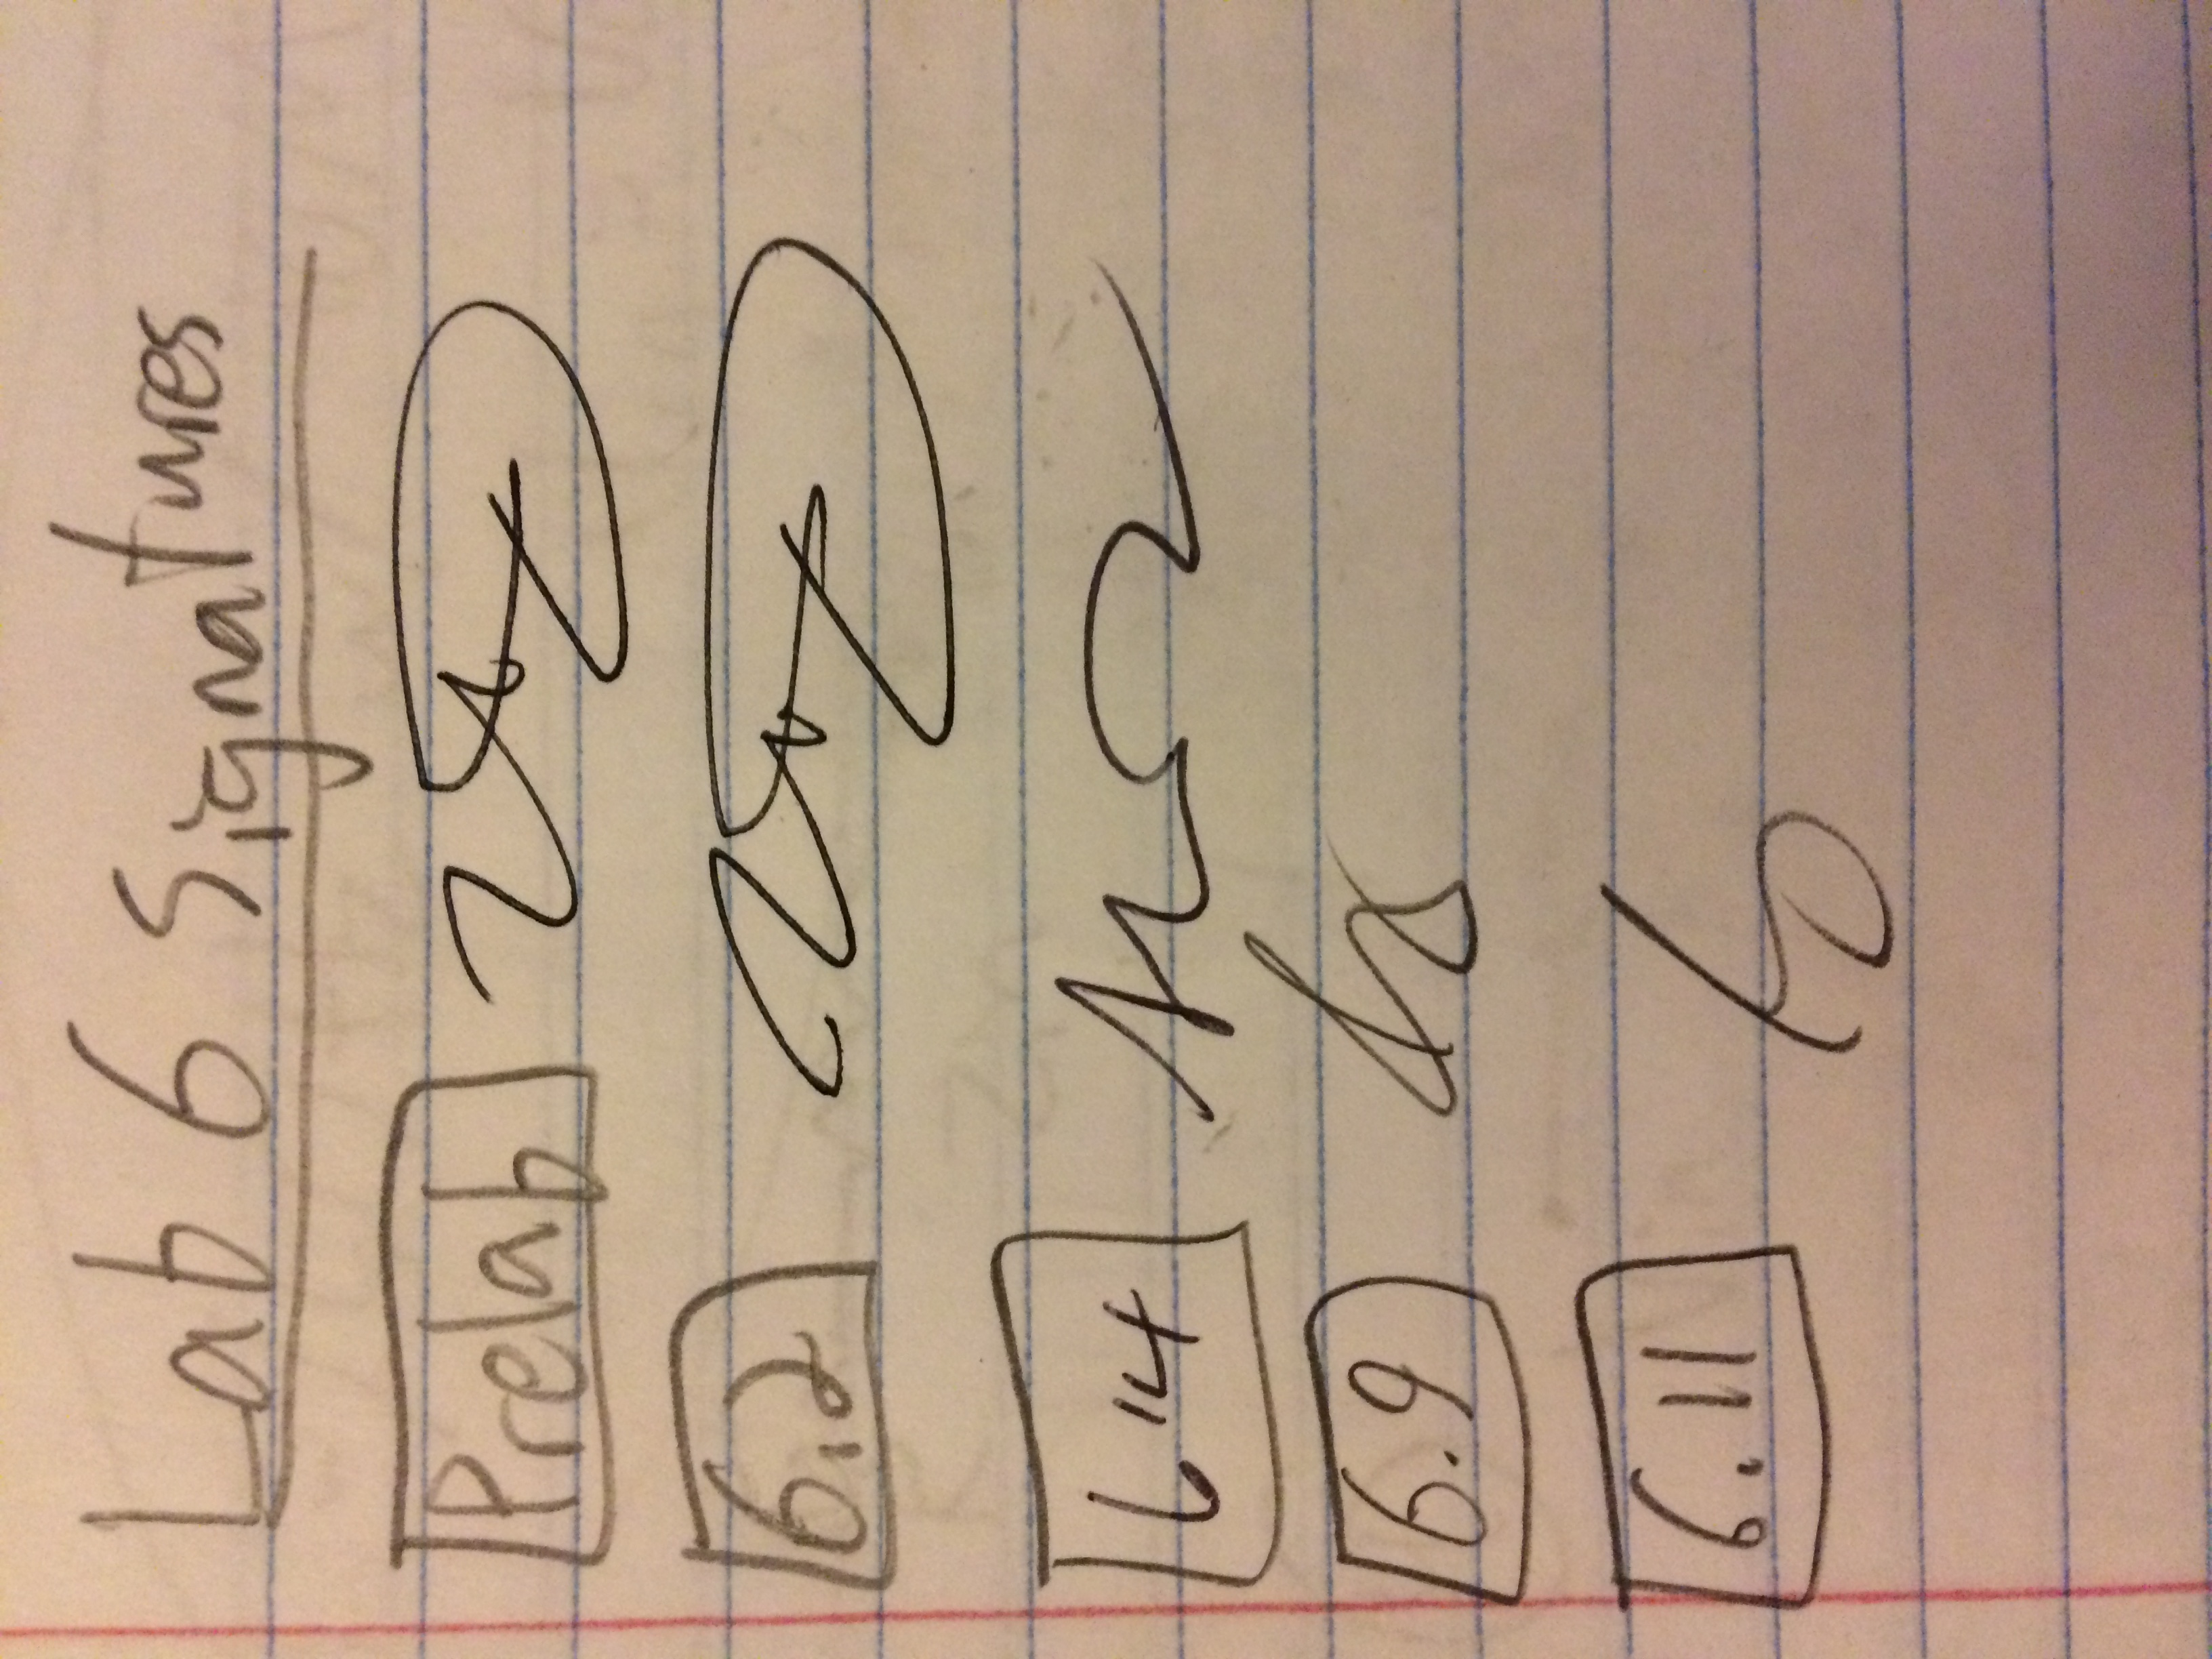
\includegraphics[scale = 0.1, angle = -90]{IMG_0239.JPG}
        \caption{Signatures for Lab 6}
        \label{fig:my_label}
    \end{figure}
    
\bibliography{joshbib}{}
\bibliographystyle{plain}

    

\end{document}


    